\documentclass[11pt,letterpaper]{article}
\usepackage[utf8]{inputenc}
\usepackage[left=1in,right=1in,top=1in,bottom=1in]{geometry}
\usepackage{amsfonts,amsmath}
\usepackage{graphicx,float}
\usepackage{esint}
\usepackage{csquotes}
% -----------------------------------
\usepackage{hyperref}
\hypersetup{%
  colorlinks=true,
  linkcolor=blue,
  citecolor=blue,
  urlcolor=blue,
  linkbordercolor={0 0 1}
}
% -----------------------------------
\usepackage[style=authoryear-icomp,backend=biber]{biblatex}
\addbibresource{citation.bib}
% -----------------------------------
\usepackage{fancyhdr}
\newcommand\course{MATH-UA.0230, PHYS-UA 180\\Introduction to Fluid Dynamics}
\newcommand\hwnumber{8}                  % <-- homework number
\newcommand\NetIDa{Ryan Sh\`iji\'e D\`u} 
\newcommand\NetIDb{March 30th, 2023}
\pagestyle{fancyplain}
\headheight 35pt
\lhead{\NetIDa\\\NetIDb}
\chead{\textbf{\Large Worksheet \hwnumber}}
\rhead{\course}
\lfoot{}
\cfoot{}
\rfoot{\small\thepage}
\headsep 1.5em
% -----------------------------------
\usepackage{titlesec}
\renewcommand\thesubsection{(\arabic{section}.\alph{subsection})}
\titleformat{\subsection}[runin]
        {\normalfont\bfseries}
        {\thesubsection}% the label and number
        {0.5em}% space between label/number and subsection title
        {}% formatting commands applied just to subsection title
        []% punctuation or other commands following subsection title
% -----------------------------------
\setlength{\parindent}{0.0in}
\setlength{\parskip}{0.1in}
% -----------------------------------
\newcommand{\de}{\mathrm{d}}
\newcommand{\DD}{\mathrm{D}}
\newcommand{\pe}{\partial}
\newcommand{\mcal}{\mathcal}
%\newcommand{\pdx}{\left|\frac{\partial}{\partial_x}\right|}

\newcommand{\dsp}{\displaystyle}

\newcommand{\norm}[1]{\left\Vert #1 \right\Vert}
%\newcommand{\mean}[1]{\left\langle #1 \right\rangle}
\newcommand{\mean}[1]{\overline{#1}}
\newcommand{\inner}[2]{\left\langle #1,#2\right\rangle}

\newcommand{\ve}[1]{\boldsymbol{#1}}

\newcommand{\thus}{\Rightarrow \quad }
\newcommand{\fff}{\iff\quad}
\newcommand{\qdt}[1]{\quad \mbox{#1} \quad}

\renewcommand{\Re}{\mathrm{Re}}
\renewcommand{\Im}{\mathrm{Im}}
\newcommand{\E}{\mathbb{E}}
\newcommand{\lap} {\nabla^2}
\renewcommand{\div}{\nabla\cdot}

\newcommand{\csch}{\text{csch}}
\newcommand{\sech}{\text{sech}}


\newcommand{\hot}{\text{h.o.t.}}

\newcommand{\ssp}{\left.\qquad\right.}

\newcommand{\var}{\text{var}}
\newcommand{\cov}{\text{cov}}


\begin{document}

\section{Examples of vorticity and circulation}
When we deal with vorticity and circulation, it is most convenient to work with polar coordinate. In (2D) polar coordinate, the vorticity (scalar) is
\begin{align}
    \omega = \frac{1}{r}\left( \frac{\pe (ru^\theta)}{\pe r}-\frac{\pe u^r}{\pe \theta} \right).
\end{align}
We will not derive this here, but a good reference is \S 5.1 and \S 5.6 of \cite{Brannon_04}. 

\subsection{Rigid body rotation}
For a body in rigid body rotation, the velocity distribution is given by
\begin{align}
    u^\theta = \Omega r \qdt{and} u^r = 0
\end{align}
where $\Omega$ is the angular velocity of the fluid (rigid body). Calculate the vorticity of this flow. How is it related to the angular velocity?

\subsection{Rankine vortex}
We have the flow field
\begin{align}
    u^\theta = \begin{cases}
        \Omega r, & r<a\\
        \dsp{\frac{\Omega a^2}{r}}, & r\geq a
    \end{cases}
\end{align}
and $u^r = 0$. 
\begin{itemize}
    \item Calculate the vorticity of this flow.
    \item Calculate the circulation of this flow around a circle with radius $R$.
\end{itemize}

\subsection{Point vortex}
We take the $a\to 0$ limit of the Rankine vortex. For this, we define $K = \Omega a^2$ and keep this a constant as we take $a$ to zero. 
\begin{itemize}
    \item How does the vorticity change as we take $a\to 0$.
    \item What is now the circulation of this flow around a circle with radius $R>a$.
\end{itemize}

\section{Point vortex velocity as a Green's function}

\subsection{Biot–Savart law}
We have the velocity field around a single point vortex. Use this and the idea of Green's function to write down the velocity field for a vortex field. This is just the 2D Biot–Savart law relating vorticity and velocity.

\subsection{Green's function for the Poisson equation}
Incompressible flow can be represented using a streamfunction $\psi$, where\footnote{sometimes it is defined with the opposite sign}
\begin{align}
    (u,v) = (-\psi_y,\psi_x). 
\end{align}

\begin{itemize}
    \item Show that the streamfunction is the solution to the Poisson equation with the vorticity on the RHS:
        \begin{align}
            \nabla^2\psi = \omega.
        \end{align}
    \item Convert the Biot–Savart law to a streamfunction. This streamfunction of the Green's function for the Poisson equation. Now you could solve the Poisson equation in $\mathbb{R}^2$.
\end{itemize}

\section{Inviscid, incompressible vortex dynamics near a wall}
Now we study inviscid, incompressible flow in the upper half plane. At the wall we use the no penetration boundary condition:
\begin{align}
    v(0,y) = 0.
\end{align}

\subsection{}
Place a point vortex into the upper plane. 
\begin{itemize}
    \item How could we make sure the flow satisfies the boundary condition?
    \item Write this in the context of the Biot–Savart law.
\end{itemize}

Hint: try placing an imaginary point vortex in the lower half plane.

\subsection{}
Think about the flow using a streamfunction. 
\begin{itemize}
    \item What is the boundary condition on the streamfunction? 
    \item Write this using the Green's function formula for the solution of the Poisson equation.
\end{itemize}

\section{Two interesting and advanced vortices examples}
\subsection{Kirchhoff Vortex} Kirchhoff vortex is a compact elliptical patch of vorticity that rotate while keeping its shape. It is a generalization of the Rankine vortex and it is the basis of study of instability. 

For details of the Kirchhoff Vortex, see \url{http://www.damtp.cam.ac.uk/user/hl278/KirchoffVortex.pdf}. For an example study of its stability, see \cite{MitchellRossi_08}.

\subsection{Lamb–Chaplygin dipole} The Lamb–Chaplygin dipole has also compact vorticity but it has positive and negative vorticity inside. It is a steady solution to the Euler equation. For more see \cite{MeleshkoHeijst_94}, image above from wikipedia.
\begin{figure}
    \centering
    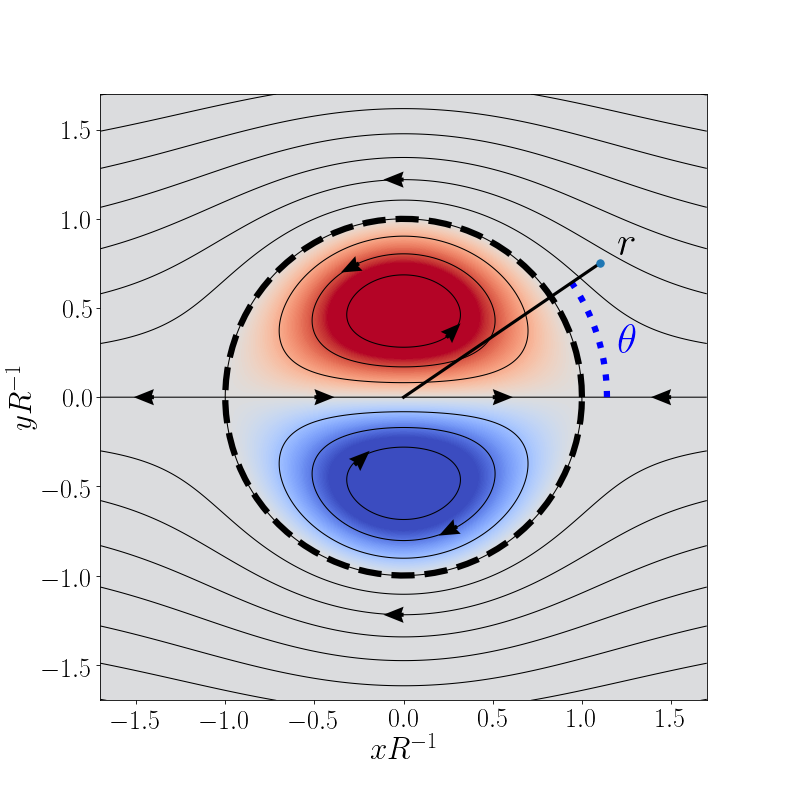
\includegraphics[width = 0.5\textwidth]{figs/Lamb-Chaplygin_dipole.png}
\end{figure}

    
\vfill
\printbibliography


\end{document}